\documentclass{article}

\usepackage{Paper}

\fancyhead[L]{EE\_ECO}
\pdftitle{Droughts}
\setlength{\droptitle}{-2.5em}

% === TITLE ===
\title{\textbf{Assignment 1 -- Droughts \\ Environmental Analysis \& Ecology}}
\author{Matteo Frongillo, Elisa Galán, Leo Koch, David Spichtig}
\date{}

% === TEXT ===
\begin{document}
\maketitle
\thispagestyle{fancy}

\vspace*{-.7cm}
\section*{The Dust Bowl event}
The Dust Bowl was a severe drought that occurred in the Great Plains region of the United States in the 1930s. It caused extreme dry conditions, dust storms, and environmental degradation in several states, particularly Oklahoma, Texas, Kansas, and Colorado. The Dust Bowl is a perfect example of how climate change can cause a severe drought in a region. 

The Dust Bowl was caused by a prolonged lack of rain in the Great Plains region of the United States. Climate change, such as ocean temperatures and atmospheric circulation, is a major cause of droughts in a region. These factors are normally affected by factors such as El Niño events. Human activities were a major cause of the Dust Bowl in the United States. Before the drought occurred, a large part of native prairie grassland was converted into agricultural land. After World War I, many farmers converted a large part of land into wheat farms, and when the drought occurred, the land became vulnerable to erosion. 

The effects of the Dust Bowl were severe. Strong winds carried large quantities of dry topsoil into the air. This resulted in massive dust storms called “black blizzards.” These blizzards caused crop loss, reduced visibility, and severe respiratory problems. There was a significant reduction in agricultural productivity. Thousands of farmers lost their livelihoods. With the loss of farms, people began to migrate to other areas in search of jobs and better living conditions. This caused significant social and economic impacts on the country. 

The Dust Bowl also experienced a number of feedback loops. Reduced rainfall resulted in low soil moisture. This reduced vegetation. This reduced vegetation increased the effects of wind erosion. The loss of fertile soil reduced the capacity to retain water. This reduced the capacity to retain vegetation. High temperatures increased the rate of evaporation. 

The disaster resulted in changes in land management and environmental policies. New programs were developed to advocate for sustainable farming practices in order to avert such calamities. Currently, the Dust Bowl disaster is an essential learning point in understanding how environmental feedback loops can create severe conditions for drought. With temperatures rising globally, such calamities might happen in other places.

\section*{Droughts from the past to the present}
Historical records show that droughts existed long before modern climate change. Thanks to multiple evidence from tree rings, lake sediments, and historical documents demonstrates that drought is a natural part of climate variability. And has ocurred many times in the past 1000 years over many parts of the world. Including: North America,  Asia, Australia and Africa.

\begin{figure}[H]
    \centering
    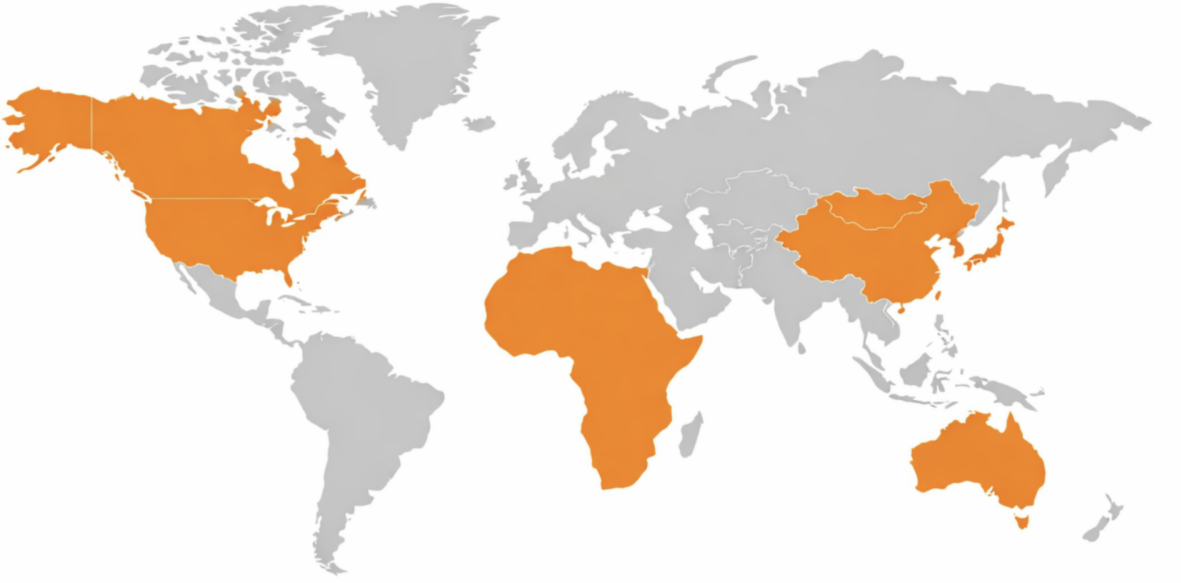
\includegraphics[width=.5\textwidth]{media/droughts_past.png}
    \caption{Regions affected by droughts in the past (including North America, Africa, East Asia, and Australia) shown in orange to indicate areas of focus in the analysis, while non-highlighted regions are displayed in grey.}
\end{figure}

\subsubsection*{Historical droughts in North America}

One of the main examples is the series of medieval megadroughts in western North America, which occurred  AD 900 and 1300. Thanks to paleoclimate records, particularly tree-ring reconstructions, we can observe that several drought periods during this time lasted 20-40 years, making them  longer than most droughts observed. Even if their intensity was comparable to more recent events like the Dust Bowl drought of the 1930s, their persistence was higher, and they occurred constantly every  400 years. Climate studies suggest that these prolonged droughts were  associated with persistent sea surface temperature patterns in the tropical Pacific Ocean, which altered atmospheric circulation and reduced precipitation over western North America, similar to La Niña conditions \parencite{wcc,aridity}. 

\subsubsection*{Historical droughts in Asia}

In East China during the period 1500-2000, archival documents and climate reconstructions indicate that droughts were more widespread and frequent than usual. 

Several severe drought episodes occurred in 1586-1589, 1638-1641, and 1965-1966, which are recognized as the most severe droughts in eastern China over the last five centuries \parencite{Shen2007ExceptionalDrought}.

These drought events showed a very particular development: they typically began in North China and gradually expanded south. The main climatic drivers are associated with changes in the East Asian summer monsoon system, particularly periods when the monsoon weakens and the Western Pacific Subtropical High shifts westward or northward. Additional contributing factors include warming in the tropical Pacific, which can weaken the summer monsoon and reduce rainfall over eastern China, as well as the potential influence of large volcanic eruptions that may temporarily alter atmospheric circulation and regional climate patterns \parencite{douville2021water}.

\subsubsection*{Historical droughts in Africa}

In West Africa during the period 1970-1980, a main example is the Sahel drought,  which caused multiple environmental and humanitarian impacts across the region. This  drought produced in widespread crop failures, water shortages, and large-scale food shortage \parencite{wcc, douville2021water}.

However, evidence from  records and other data suggests that similarly severe dry and wet periods have happened repeatedly in the region over the past three millennia, indicating that the Sahel drought was not unprecedented in the long-term climate context \parencite{aridity}.

Scientific studies suggest that these drought conditions are responsible primarily due to changes in sea surface temperatures in the tropical Atlantic Ocean, which caused a reduction of rainfall across the Sahel. Additional influences like Land-surface processes may also amplify drought conditions, creating a reinforcing effect that increases the intensity and duration of the drought episodes \parencite{wcc, douville2021water}.

\subsubsection*{Historical droughts in Australia}
Australia has experienced several major historical droughts, with one of the most significant being the Federation Drought (1895-1903), followed by the World War II drought (1937-1945) and the more recent Millennium Drought (1997-2009). These droughts affected large parts of the continent, particularly southeastern and eastern Australia, leading to severe water shortages, agricultural losses, and ecosystem stress. Paleoclimate reconstructions based on tree rings, coral records, and sediment data indicate that drought variability in Australia extends well beyond the instrumental record, with evidence of prolonged dry periods over the past several centuries. The Millennium Drought, for example, was characterized by persistently low rainfall and reduced river inflows in the Murray-Darling Basin, making it one of the most severe droughts in terms of water resource impact \parencite{BOMWhatIsDrought}.

\section*{Future droughts scenarios}
Drought is expected to become an increasingly serious environmental and social issue in the future as global climate change continues to influence weather patterns and temperature levels. Although drought is commonly understood as a period of unusually low rainfall, it is also strongly connected to rising temperatures, which increase evaporation and reduce soil moisture. As a result, land can become drier more quickly, even in regions where annual precipitation does not decrease significantly. This suggests that future droughts may not only occur more often, but may also become longer-lasting and more intense. In many parts of the world, especially those already vulnerable to dry conditions, the risk of persistent drought is likely to grow during the coming decades. 

One major future scenario is the increasing pressure on water resources, agriculture, and economic stability. Lower water availability in rivers, lakes, and reservoirs may affect drinking water supplies, energy production, and industrial activity. At the same time, agriculture will face significant challenges because crop growth depends heavily on reliable water access. Extended dry periods can reduce soil fertility, lower agricultural yields, and threaten food security, particularly in regions that depend on seasonal rainfall. In addition, farmers may be forced to adapt by changing planting times, switching to more drought-resistant crops, or investing in costly irrigation systems. These changes could place a particularly heavy burden on poorer regions, where financial resources, technology, and water infrastructure are often limited. Therefore, the future effects of drought are not only environmental, but also economic and social. 

A further important scenario concerns the impact of drought on ecosystems and general living conditions. Forests, grasslands, and wetlands are highly sensitive to prolonged water shortages, and many animal and plant species may struggle to survive under increasingly dry conditions. Drought can also increase the likelihood of wildfires, desertification, and long-term damage to natural habitats. In human societies, these environmental pressures may lead to migration, conflict over water resources, and greater inequality between regions that are able to adapt and those that are not. For this reason, future responses to drought will require careful planning and long-term strategies. Improved water management, more efficient agricultural systems, early warning technologies, and climate adaptation policies will be essential in reducing the damage caused by future drought events. Overall, drought is likely to become more widespread, more severe, and more disruptive, making it a critical challenge for both present and future generations. 

\section*{Mixed-grass prairies after the Dust Bowl}
In the 1930s, a severe drought struck the Great Plains region of North Dakota, leading to a prolonged period of no rainfall and frequent dust storms. The Dust Bowl was the main cause of this multi-year drought, which resulted in a sharp decline in precipitation, raising temperatures, and creating strong winds \parencite{ndmc_dust_bowl}. With a PDSI of - 3 to -4 or less, the Great Plains drought reached “severe to extreme” levels [\autoref{appendix:PDSI}], [\autoref{fig:PDSI}]. 
\begin{figure}[ht!]
    \centering
    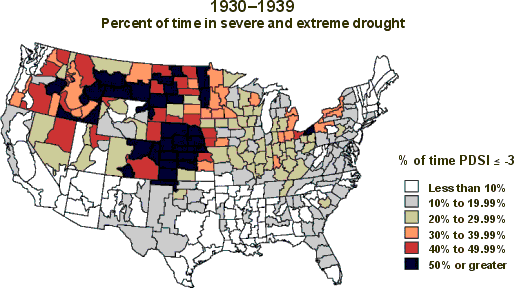
\includegraphics[width=.65\textwidth]{media/PDSI_dustbowl.png}
    \caption{PDSI values during the U.S. Dust Bowl, 1930-39 \parencite{mata_dust_bowl_pdsi_figure}.}
    \label{fig:PDSI}
\end{figure}

Before the Dust Bowl, North Dakota’s mixed-grass prairie was a strong semi-arid ecosystem with rolling plains, fertile soil, and a continental climate (long, cold winters; hot, dry summers; and about 25-50 cm of rain each year) \parencite{northwestern_great_plains_mixed_grass_prairie_2020}. This prairie includes shortgrass and tallgrass biomes. It is mostly made up of a mix of warm-season and cool-season grasses. Bison, antelope, and prairie dogs and birds were some of the animals that lived in the grassland \parencite{northwestern_great_plains_mixed_grass_prairie_2020}. Drought, wildfires, and grazing by native species were all natural events that happened from time to time, and the ecosystem had adapted well to them when it was still intact. 

The drought had a huge negative impact on this prairie ecosystem: plant-available soil moisture dropped to a record lows because there was almost no effective rain for two growing seasons in a row. Taking away the protective plant cover made the loose topsoil more likely to erode. Strong winds moved the dry soils, creating huge dust storms that swept away fine particles and nutrient-rich topsoil \parencite{droughts_pdf}. Millions of tons of topsoil were blown away from North Dakota’s prairies, which caused long-term damage to the soil’s ability to grow plants. The fauna was very affected by the runout of forage, and livestock and wild herbivores that grazed on it starved to death or were moved. Prairie dogs lost food and saw their colonies die off. Water sources dried up, important wetlands shrank, and animals died because they lost places to breed. By the end of the 30s, a lot of what had been productive prairie had turned into a barren landscape covered in dust. The ecosystem fell apart, and topsoil retention, carbon sequestration, and nutrient cycling all got a lot worse \parencite{sanderson2015longterm}.

\section*{Casual Loop Diagram (CLD) of drought in prairie ecosystems}
\begin{figure}[H]
    \centering
    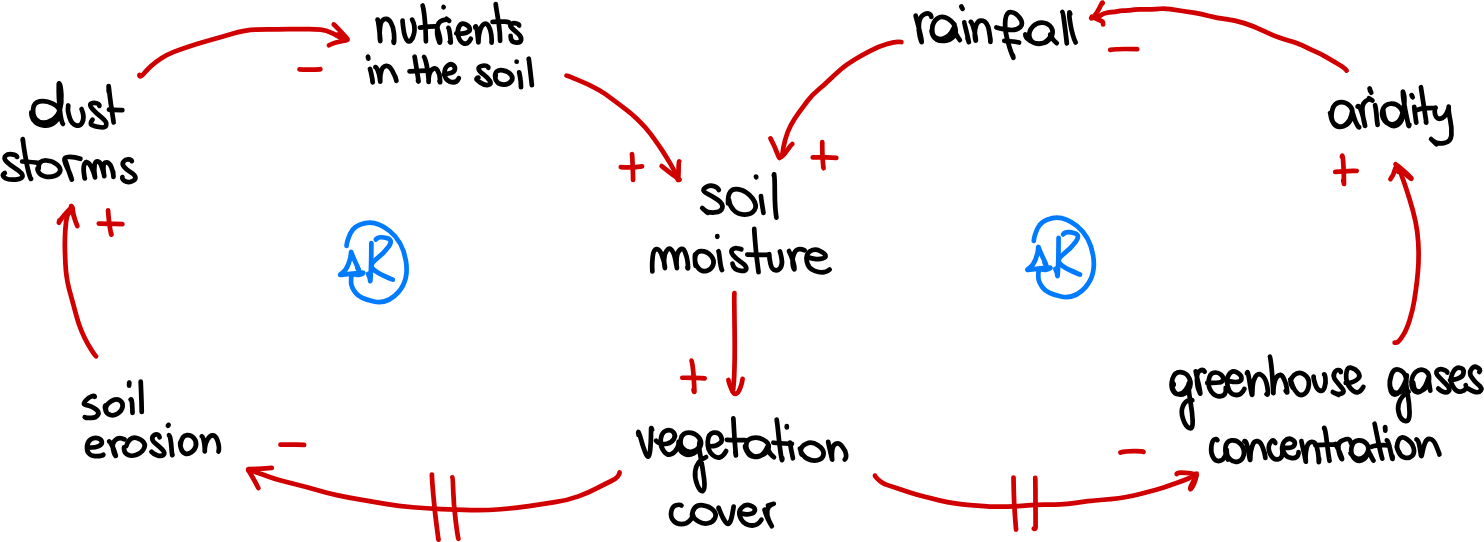
\includegraphics[width=.8\textwidth]{media/CLD.png}
    \caption{Droughts modeled as a Casual Loop Diagram (CLD)}
\end{figure}

This causal loop diagram shows how drought can intensify through a set of connected environmental processes. The central variable is soil moisture, because it directly affects vegetation cover. When soil moisture decreases, vegetation cover also decreases because plants have less water available to survive and grow. 

Vegetation cover is important because it helps protect the land. It has a negative relationship with both soil erosion and greenhouse gas concentration. This means that when vegetation cover goes down, soil erosion goes up, and greenhouse gas concentration also increases. These changes then trigger two reinforcing feedback loops that make drought conditions worse over time. 

In the first reinforcing loop, less vegetation cover leads to greater soil erosion. Analogously to the first reinforcing loop, the vegetation growth and death cycle leads to a time delay to soil erosion. Increased soil erosion causes more dust storms, and more dust storms reduce nutrients in the soil. With fewer nutrients in the soil, the land becomes less able to retain and support soil moisture. As soil moisture decreases further, vegetation cover declines even more, which strengthens the cycle. This loop shows how land degradation can reinforce drought. 

In the second reinforcing loop, lower vegetation cover leads to a higher greenhouse gas concentration. The increase in greenhouse gas concentration is not instantaneous: vegetation generally has a long growth and death cycle if not influenced by external factors, so the capture of greenhouse gas and, consequently, its release, is not immediate and requires the inclusion of a time delay. Higher greenhouse gas concentration increases aridity, meaning the environment becomes hotter and drier. Greater aridity reduces rainfall, and less rainfall lowers soil moisture. As soil moisture drops, vegetation cover continues to decline, which further increases greenhouse gas concentration. This creates another reinforcing cycle that worsens drought conditions. 

Overall, the diagram explains that drought is not just caused by one single factor. Instead, it is strengthened by interconnected feedback loops involving vegetation loss, soil degradation, reduced rainfall, and increasing aridity. Because both loops are reinforcing loops, any initial decrease in soil moisture can set off a chain reaction that makes the drought more severe over time.

\subsubsection*{Reference Behavior Pattern (RBP)}
\begin{figure}[H]
    \centering
    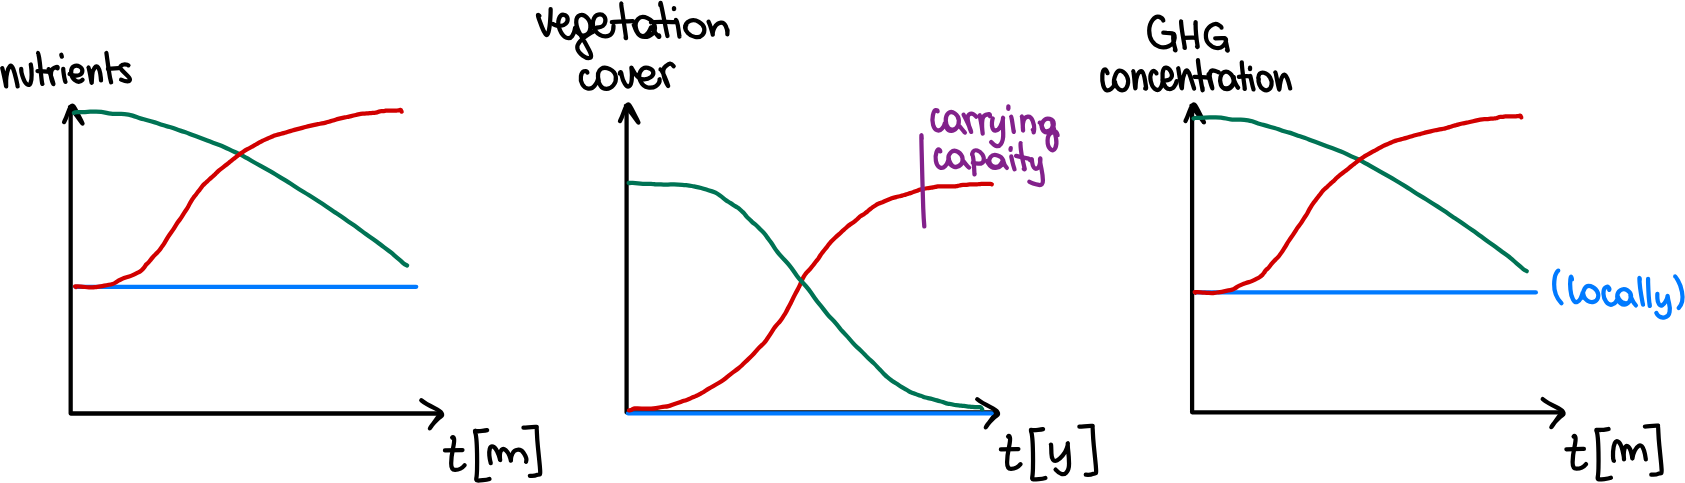
\includegraphics[width=\textwidth]{media/RBPs.png}
    \caption{RBPs of nutrients in the soil, vegetation cover, and greenhouse gases concentration as the modeled variables}
\end{figure}

Because both modeled loops are reinforcing loops, each variable exhibits one of three trends:
\begin{enumerate}
    \item the variable tends to grow exponentially without limit;
    \item the variable decays exponentially until it reaches zero;
    \item the variable remains constant.
\end{enumerate}

In the case of the modeled CLD, the variables chosen were nutrients, vegetation cover, and greenhouse gas concentration. Vegetation cover was chosen because it is at the center of the graph and is the variable that enables the strengthening or weakening of the entire modeled system, that is drought. Nutrients were chosen because they are key to vegetation growth and effectively demonstrate how drought affects them. Finally, greenhouse gas concentration shows how, locally, the intensification of greenhouse gases, resulting in rising temperatures and reduced rainfall, may or may not intensify drought. 

The considerations made in designing the three graphs are as follows:

Nutrients: There are no external influences, and nutrient levels are based solely on the soil under consideration. The modeling time span is measured in months because plants do not appear and die instantly; rather, soil erosion and the resulting nutrient cycling in the soil are slow processes.

Vegetation cover: The area covered by vegetation is limited, resulting in a carrying capacity that prevents the graph from growing indefinitely.
The time axis is expressed in years, and it is assumed that there are no drastic increases or decreases due to seasonal changes.

Greenhouse gas concentration: Similar to soil nutrients, this variable is modeled solely at the local level and does not account for external factors that could potentially alter the concentration in the environment. Time is shown in months because the process of vegetation growth and decay is slow; consequently, the increase in concentration itself is also slow.

\newpage
\appendix
\part*{Appendix}
\section{PDSI table}
\label{appendix:PDSI}
\begin{table}[ht!]
    \caption*{Extract from Table 1 ``Comparison of Commonly-used Drought Indice'' \parencite{droughts_pdf}}
    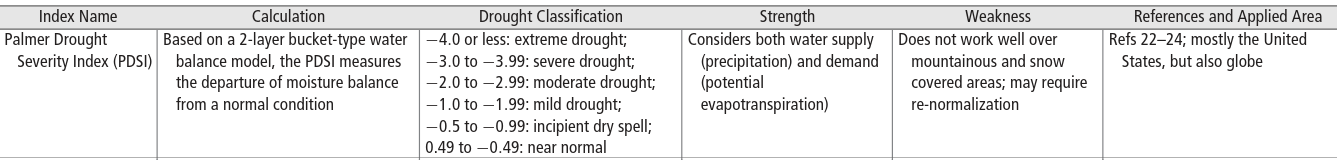
\includegraphics[width=\textwidth]{media/PDSI_table.png}
    \label{table:PDSI}
\end{table}

\setlength{\bibitemsep}{1.2\baselineskip}
\begin{refcontext}[sorting=none]
    \printbibliography[title=B\hspace*{.4cm} References]
\end{refcontext}









\end{document}
